\section{Pretrained model evaluation}

\subsection{Per-benchmark results}\label{appendix:full_results_pretraining}

\begin{table}
\centering
\begin{NiceTabular}{lcccc}
	\CodeBefore
	\Body
	\toprule
	& \multicolumn{3}{c}{\textbf{Reading Comprehension}} \\
	\midrule
	& SQuAD & QuAC & RACE & \textit{Winrate}\\
\cmidrule{2-4}
	Llama 3 8B & 77.0 \scriptsize{$\pm$0.8}& \textbf{44.9 \scriptsize{$\pm$1.1}}& \textbf{54.3 \scriptsize{$\pm$1.4}} & \textit{2}\\
	Llama 2 7B &72.3 \scriptsize{$\pm$0.8}& 39.5 \scriptsize{$\pm$1.1}& 51.1 \scriptsize{$\pm$1.4} & \textit{0}\\
	Llama 2 13B &72.2 \scriptsize{$\pm$0.8}& \textbf{44.9 \scriptsize{$\pm$1.1}}& \textbf{53.9 \scriptsize{$\pm$1.4}} & \textit{2}\\
	Mistral 7B &73.2 \scriptsize{$\pm$0.8}& \textbf{44.7 \scriptsize{$\pm$1.1}}& \textbf{53.0 \scriptsize{$\pm$1.4}} & \textit{2}\\
	Gemma 7B &\textbf{81.8 \scriptsize{$\pm$0.7}}& 42.4 \scriptsize{$\pm$1.1}& 48.8 \scriptsize{$\pm$1.4} & \textit{1}\\
	\cmidrule{2-4}
	Llama 3 70B & 81.8 \scriptsize{$\pm$0.7}& \textbf{51.1 \scriptsize{$\pm$1.1}}& \textbf{59.0 \scriptsize{$\pm$1.4}} & \textit{2}\\
	Mixtral 8x22B &\textbf{84.1 \scriptsize{$\pm$0.7}}& 44.9 \scriptsize{$\pm$1.1}& \textbf{59.2 \scriptsize{$\pm$1.4}} & \textit{2}\\
	Qwen2 72B &73.2 \scriptsize{$\pm$0.8}& \textbf{51.1 \scriptsize{$\pm$1.1}}& \textbf{60.8 \scriptsize{$\pm$1.4}} & \textit{2}\\
	Llama 2 70B &82.6 \scriptsize{$\pm$0.7}& \textbf{49.5 \scriptsize{$\pm$1.1}}& 56.2 \scriptsize{$\pm$1.4} & \textit{1}\\
	\cmidrule{2-4}
	Llama 3 405B & \textbf{81.8 \scriptsize{$\pm$0.7}}& \textbf{53.6 \scriptsize{$\pm$1.1}}& \textbf{58.1 \scriptsize{$\pm$1.4}} & \textit{3}\\
	GPT4 &-& -& - & \textit{0}\\
	Nemotron &-& -& - & \textit{0}\\
	Gemini Ultra &-& -& - & \textit{0}\\
	\bottomrule
\end{NiceTabular}

\caption{Non-aggregated pretraining evaluation results for the Knowledge and Reasoning categories.}
\label{table:full_results_pretraining_reading_comprehension}
\end{table}

\begin{table}
\centering
\begin{NiceTabular}{lccc}
	\CodeBefore
	\Body
	\toprule
	& \multicolumn{2}{c}{\textbf{Knowledge}} \\
	\midrule
	& TriviaQA & TruthfulQA & \textit{Winrate}\\
\cmidrule{2-3}
	Llama 3 8B & 77.6 \scriptsize{$\pm$0.8}& \textbf{44.1 \scriptsize{$\pm$3.4}} & \textit{1}\\
	Llama 2 7B &72.1 \scriptsize{$\pm$0.8}& \textbf{38.7 \scriptsize{$\pm$3.3}} & \textit{1}\\
	Llama 2 13B &\textbf{79.6 \scriptsize{$\pm$0.7}}& 37.3 \scriptsize{$\pm$3.3} & \textit{1}\\
	Mistral 7B &76.6 \scriptsize{$\pm$0.8}& \textbf{41.7 \scriptsize{$\pm$3.4}} & \textit{1}\\
	Gemma 7B &72.6 \scriptsize{$\pm$0.8}& \textbf{45.1 \scriptsize{$\pm$3.4}} & \textit{1}\\
	\cmidrule{2-3}
	Llama 3 70B & \textbf{89.8 \scriptsize{$\pm$0.6}}& \textbf{51.0 \scriptsize{$\pm$3.4}} & \textit{2}\\
	Mixtral 8x22B &\textbf{88.8 \scriptsize{$\pm$0.6}}& \textbf{51.1 \scriptsize{$\pm$3.4}} & \textit{2}\\
	Qwen2 72B &85.6 \scriptsize{$\pm$0.6}& \textbf{54.8 \scriptsize{$\pm$3.4}} & \textit{1}\\
	Llama 2 70B &87.7 \scriptsize{$\pm$0.6}& 44.9 \scriptsize{$\pm$3.4} & \textit{0}\\
	\cmidrule{2-3}
	Llama 3 405B & \textbf{91.8 \scriptsize{$\pm$0.5}}& \textbf{49.7 \scriptsize{$\pm$3.4}} & \textit{2}\\
	GPT4 &-& - & \textit{0}\\
	Nemotron &-& - & \textit{0}\\
	Gemini Ultra &-& - & \textit{0}\\
	\bottomrule
\end{NiceTabular}

\caption{Non-aggregated pretraining evaluation results for the Knowledge and Reasoning categories.}
\label{table:full_results_pretraining_knowledge}
\end{table}

\begin{table}
\centering
\begin{NiceTabular}{lcccccc}
	\CodeBefore
	\Body
	\toprule
	& \multicolumn{5}{c}{\textbf{Commonsense}} \\
	\midrule
	& CommonSenseQA & PiQA & SiQA & OpenBookQA & WinoGrande & \textit{Winrate}\\
\cmidrule{2-6}
	Llama 3 8B & \textbf{75.0 \scriptsize{$\pm$2.5}}& \textbf{81.0 \scriptsize{$\pm$1.8}}& \textbf{49.5 \scriptsize{$\pm$2.2}}& \textbf{45.0 \scriptsize{$\pm$4.4}}& \textbf{75.7 \scriptsize{$\pm$2.0}} & \textit{5}\\
	Llama 2 7B &57.9 \scriptsize{$\pm$2.9}& 78.9 \scriptsize{$\pm$1.9}& \textbf{48.4 \scriptsize{$\pm$2.2}}& \textbf{44.4 \scriptsize{$\pm$4.4}}& 73.0 \scriptsize{$\pm$2.1} & \textit{2}\\
	Llama 2 13B &67.4 \scriptsize{$\pm$2.7}& \textbf{80.4 \scriptsize{$\pm$1.8}}& \textbf{50.6 \scriptsize{$\pm$2.2}}& \textbf{44.8 \scriptsize{$\pm$4.4}}& \textbf{75.9 \scriptsize{$\pm$2.0}} & \textit{4}\\
	Mistral 7B &\textbf{71.2 \scriptsize{$\pm$2.6}}& \textbf{83.0 \scriptsize{$\pm$1.7}}& \textbf{48.2 \scriptsize{$\pm$2.2}}& \textbf{47.8 \scriptsize{$\pm$4.4}}& \textbf{78.1 \scriptsize{$\pm$1.9}} & \textit{5}\\
	Gemma 7B &\textbf{74.4 \scriptsize{$\pm$2.5}}& \textbf{81.5 \scriptsize{$\pm$1.8}}& \textbf{51.8 \scriptsize{$\pm$2.2}}& \textbf{52.8 \scriptsize{$\pm$4.4}}& \textbf{74.7 \scriptsize{$\pm$2.0}} & \textit{5}\\
	\cmidrule{2-6}
	Llama 3 70B & 84.1 \scriptsize{$\pm$2.1}& \textbf{83.8 \scriptsize{$\pm$1.7}}& 52.2 \scriptsize{$\pm$2.2}& \textbf{47.6 \scriptsize{$\pm$4.4}}& \textbf{83.5 \scriptsize{$\pm$1.7}} & \textit{3}\\
	Mixtral 8x22B &82.4 \scriptsize{$\pm$2.2}& \textbf{85.5 \scriptsize{$\pm$1.6}}& 51.6 \scriptsize{$\pm$2.2}& \textbf{50.8 \scriptsize{$\pm$4.4}}& \textbf{84.7 \scriptsize{$\pm$1.7}} & \textit{3}\\
	Qwen2 72B &\textbf{90.5 \scriptsize{$\pm$1.7}}& \textbf{83.6 \scriptsize{$\pm$1.7}}& \textbf{62.5 \scriptsize{$\pm$2.1}}& \textbf{49.0 \scriptsize{$\pm$4.4}}& \textbf{85.1 \scriptsize{$\pm$1.7}} & \textit{5}\\
	Llama 2 70B &78.9 \scriptsize{$\pm$2.4}& \textbf{82.5 \scriptsize{$\pm$1.7}}& 50.8 \scriptsize{$\pm$2.2}& \textbf{49.2 \scriptsize{$\pm$4.4}}& \textbf{82.2 \scriptsize{$\pm$1.8}} & \textit{3}\\
	\cmidrule{2-6}
	Llama 3 405B & \textbf{85.8 \scriptsize{$\pm$2.0}}& \textbf{85.6 \scriptsize{$\pm$1.6}}& \textbf{53.7 \scriptsize{$\pm$2.2}}& \textbf{49.2 \scriptsize{$\pm$4.4}}& 82.2 \scriptsize{$\pm$1.8} & \textit{4}\\
	GPT4 &-& -& -& -& \textbf{87.5 \scriptsize{$\pm$1.5}} & \textit{1}\\
	Nemotron &-& -& -& -& \textbf{89.5 \scriptsize{$\pm$1.4}} & \textit{1}\\
	Gemini Ultra &-& -& -& -& - & \textit{0}\\
	\bottomrule
\end{NiceTabular}

\caption{Non-aggregated pretraining evaluation results for the Commonsense reasoning and understanding benchmarks.}
\label{table:full_results_pretraining_commonsense}
\end{table}

\begin{table}
\centering
\begin{NiceTabular}{lcccccc}
	\CodeBefore
	\Body
	\toprule
	& \multicolumn{5}{c}{\textbf{Math and Reasoning}} \\
	\midrule
	& GSM8K & MATH & ARC-C & DROP & WorldSense & \textit{Winrate}\\
\cmidrule{2-6}
	Llama 3 8B & \textbf{57.2 \scriptsize{$\pm$2.7}}& 20.3 \scriptsize{$\pm$1.1}& \textbf{79.7 \scriptsize{$\pm$2.3}}& \textbf{59.5 \scriptsize{$\pm$1.0}}& \textbf{45.5 \scriptsize{$\pm$0.3}} & \textit{4}\\
	Llama 2 7B &14.9 \scriptsize{$\pm$1.9}& 3.0 \scriptsize{$\pm$0.5}& 54.6 \scriptsize{$\pm$2.9}& 40.5 \scriptsize{$\pm$1.0}& 44.4 \scriptsize{$\pm$0.3} & \textit{0}\\
	Llama 2 13B &29.3 \scriptsize{$\pm$2.5}& 5.2 \scriptsize{$\pm$0.6}& 67.0 \scriptsize{$\pm$2.7}& 49.7 \scriptsize{$\pm$1.0}& 44.5 \scriptsize{$\pm$0.3} & \textit{0}\\
	Mistral 7B &\textbf{52.5 \scriptsize{$\pm$2.7}}& 13.1 \scriptsize{$\pm$0.9}& \textbf{78.2 \scriptsize{$\pm$2.4}}& 53.0 \scriptsize{$\pm$1.0}& 44.9 \scriptsize{$\pm$0.3} & \textit{2}\\
	Gemma 7B &46.4 \scriptsize{$\pm$2.7}& \textbf{24.3 \scriptsize{$\pm$1.2}}& \textbf{78.6 \scriptsize{$\pm$2.4}}& 56.3 \scriptsize{$\pm$1.0}& \textbf{46.0 \scriptsize{$\pm$0.3}} & \textit{3}\\
	\cmidrule{2-6}
	Llama 3 70B & 83.7 \scriptsize{$\pm$2.0}& 41.4 \scriptsize{$\pm$1.4}& \textbf{92.9 \scriptsize{$\pm$1.5}}& \textbf{79.6 \scriptsize{$\pm$0.8}}& 61.1 \scriptsize{$\pm$0.3} & \textit{2}\\
	Mixtral 8x22B &\textbf{88.4 \scriptsize{$\pm$1.7}}& 41.8 \scriptsize{$\pm$1.4}& 91.9 \scriptsize{$\pm$1.6}& 77.5 \scriptsize{$\pm$0.8}& 51.5 \scriptsize{$\pm$0.3} & \textit{1}\\
	Qwen2 72B &\textbf{89.5 \scriptsize{$\pm$1.7}}& \textbf{55.9 \scriptsize{$\pm$1.4}}& \textbf{95.0 \scriptsize{$\pm$1.2}}& 76.9 \scriptsize{$\pm$0.8}& \textbf{68.2 \scriptsize{$\pm$0.3}} & \textit{4}\\
	Llama 2 70B &57.9 \scriptsize{$\pm$2.7}& 13.6 \scriptsize{$\pm$1.0}& 85.4 \scriptsize{$\pm$2.0}& 70.1 \scriptsize{$\pm$0.9}& 45.5 \scriptsize{$\pm$0.3} & \textit{0}\\
	\cmidrule{2-6}
	Llama 3 405B & \textbf{89.0 \scriptsize{$\pm$1.7}}& \textbf{53.8 \scriptsize{$\pm$1.4}}& \textbf{96.1 \scriptsize{$\pm$1.1}}& \textbf{84.8 \scriptsize{$\pm$0.7}}& \textbf{63.7 \scriptsize{$\pm$0.3}} & \textit{5}\\
	GPT4 &\textbf{92.0 \scriptsize{$\pm$1.5}}& -& \textbf{96.3 \scriptsize{$\pm$1.1}}& 80.9 \scriptsize{$\pm$0.8}& - & \textit{2}\\
	Nemotron &-& -& \textbf{94.3 \scriptsize{$\pm$1.3}}& -& - & \textit{1}\\
	Gemini Ultra &\textbf{88.9 \scriptsize{$\pm$1.7}}& \textbf{53.2 \scriptsize{$\pm$1.4}}& -& 82.4 \scriptsize{$\pm$0.8}& - & \textit{2}\\
	\bottomrule
\end{NiceTabular}

\caption{Non-aggregated pretraining evaluation results for math and reasoning benchmarks.}
\label{table:full_results_math_reasoning}
\end{table}

\begin{table}
\centering
\begin{NiceTabular}{lccc}
	\CodeBefore
	\Body
	\toprule
	& \multicolumn{2}{c}{\textbf{Code}} \\
	\midrule
	& HumanEval & MBPP & \textit{Winrate}\\
\cmidrule{2-3}
	Llama 3 8B & \textbf{37.2 \scriptsize{$\pm$7.4}}& \textbf{47.6 \scriptsize{$\pm$4.4}} & \textit{2}\\
	Llama 2 7B &12.8 \scriptsize{$\pm$5.1}& 22.0 \scriptsize{$\pm$3.6} & \textit{0}\\
	Llama 2 13B &18.9 \scriptsize{$\pm$6.0}& 27.6 \scriptsize{$\pm$3.9} & \textit{0}\\
	Mistral 7B &\textbf{30.5 \scriptsize{$\pm$7.0}}& \textbf{47.5 \scriptsize{$\pm$4.4}} & \textit{2}\\
	Gemma 7B &\textbf{32.3 \scriptsize{$\pm$7.2}}& \textbf{44.4 \scriptsize{$\pm$4.4}} & \textit{2}\\
	\cmidrule{2-3}
	Llama 3 70B & \textbf{58.5 \scriptsize{$\pm$7.5}}& 66.2 \scriptsize{$\pm$4.1} & \textit{1}\\
	Mixtral 8x22B &45.1 \scriptsize{$\pm$7.6}& \textbf{71.2 \scriptsize{$\pm$4.0}} & \textit{1}\\
	Qwen2 72B &\textbf{64.6 \scriptsize{$\pm$7.3}}& \textbf{76.9 \scriptsize{$\pm$3.7}} & \textit{2}\\
	Llama 2 70B &29.3 \scriptsize{$\pm$7.0}& 45.2 \scriptsize{$\pm$4.4} & \textit{0}\\
	\cmidrule{2-3}
	Llama 3 405B & 61.0 \scriptsize{$\pm$7.5}& \textbf{73.4 \scriptsize{$\pm$3.9}} & \textit{1}\\
	GPT4 &67.0 \scriptsize{$\pm$7.2}& - & \textit{0}\\
	Nemotron &57.3 \scriptsize{$\pm$7.6}& - & \textit{0}\\
	Gemini Ultra &\textbf{74.4 \scriptsize{$\pm$4.2}}& - & \textit{1}\\
	\bottomrule
\end{NiceTabular}

    \caption{Non-aggregated pretraining evaluation results for long context (\TBD{still missing}) and code.}
\label{table:full_results_code}
\end{table}

\begin{table}
\centering
    \begin{NiceTabular}{lccccc}
	\CodeBefore
	\Body
	\toprule
	& \multicolumn{4}{c}{\textbf{General}} \\
	\midrule
	& MMLU & MMLU-Pro & AGIEval & BIG-Bench Hard & \textit{Winrate}\\
\cmidrule{2-5}
	Llama 3 8B & \textbf{65.6 \scriptsize{$\pm$0.8}}& \textbf{35.6 \scriptsize{$\pm$0.9}}& \textbf{47.8 \scriptsize{$\pm$1.9}}& \textbf{64.2 \scriptsize{$\pm$1.2}} & \textit{4}\\
	Llama 2 7B &45.7 \scriptsize{$\pm$0.8}& 18.9 \scriptsize{$\pm$0.7}& 29.1 \scriptsize{$\pm$1.8}& 39.0 \scriptsize{$\pm$1.2} & \textit{0}\\
	Llama 2 13B &55.4 \scriptsize{$\pm$0.8}& 23.8 \scriptsize{$\pm$0.8}& 38.6 \scriptsize{$\pm$1.9}& 46.9 \scriptsize{$\pm$1.2} & \textit{0}\\
	Mistral 7B &62.5 \scriptsize{$\pm$0.8}& 30.7 \scriptsize{$\pm$0.8}& 42.7 \scriptsize{$\pm$1.9}& 56.8 \scriptsize{$\pm$1.2} & \textit{0}\\
	Gemma 7B &\textbf{64.3 \scriptsize{$\pm$0.8}}& 33.6 \scriptsize{$\pm$0.8}& \textbf{46.0 \scriptsize{$\pm$1.9}}& 57.7 \scriptsize{$\pm$1.2} & \textit{2}\\
	\cmidrule{2-5}
	Llama 3 70B & 79.0 \scriptsize{$\pm$0.7}& 52.0 \scriptsize{$\pm$0.9}& 64.6 \scriptsize{$\pm$1.9}& \textbf{81.6 \scriptsize{$\pm$0.9}} & \textit{1}\\
	Mixtral 8x22B &77.8 \scriptsize{$\pm$0.7}& 49.9 \scriptsize{$\pm$0.9}& 61.5 \scriptsize{$\pm$1.9}& 79.5 \scriptsize{$\pm$1.0} & \textit{0}\\
	Qwen2 72B &\textbf{84.3 \scriptsize{$\pm$0.6}}& \textbf{55.8 \scriptsize{$\pm$0.9}}& \textbf{72.4 \scriptsize{$\pm$1.7}}& \textbf{82.4 \scriptsize{$\pm$0.9}} & \textit{4}\\
	Llama 2 70B &69.1 \scriptsize{$\pm$0.8}& 37.0 \scriptsize{$\pm$0.9}& 53.6 \scriptsize{$\pm$1.9}& 65.7 \scriptsize{$\pm$1.2} & \textit{0}\\
	\cmidrule{2-5}
	Llama 3 405B & \textbf{85.4 \scriptsize{$\pm$0.6}}& \textbf{59.6 \scriptsize{$\pm$0.9}}& \textbf{71.6 \scriptsize{$\pm$1.8}}& \textbf{85.9 \scriptsize{$\pm$0.8}} & \textit{4}\\
	GPT4 &\textbf{86.4 \scriptsize{$\pm$0.6}}& -& -& - & \textit{1}\\
	Nemotron &81.1 \scriptsize{$\pm$0.6}& -& -& \textbf{85.4 \scriptsize{$\pm$0.9}} & \textit{1}\\
	Gemini Ultra &83.7 \scriptsize{$\pm$0.6}& -& -& 83.6 \scriptsize{$\pm$0.9} & \textit{0}\\
	\bottomrule
\end{NiceTabular}

    \caption{Non-aggregated pretraining evaluation results for aggregate benchmarks.}
\label{table:full_results_general}
\end{table}


\section{Reproducibility: Prompts and fewshots examples}\label{appendix:prompt_details}

\begin{table}[]
\small
\centering
\setlength{\tabcolsep}{1.5pt}
\begin{tabular}{lcccc}
\toprule
\small
\bfseries Benchmark & \bfseries License & \bfseries \# samples & \bfseries \# few-shot & \bfseries Metric \\
\midrule
\makecell[l]{Adv SQuAD \citep{jia-liang-2017-adversarial}} & &  & 1 &  F1 \\
\midrule
\makecell[l]{AGIEval \citep{zhong2023agieval}} & MIT & 2546 & 3-5 & Accuracy \\
\midrule
\makecell[l]{ARC-C \citep{clark2018think}} & Apache 2.0 & 1165 & 0 & Accuracy \\
\midrule
\makecell[l]{Big Bench Hard \citep{suzgun-etal-2023-challenging}} & Apache 2.0 &  6511 & 3 (CoT) & EM (micro avg) \\
\midrule
\makecell[l]{CommonSenseQA \\\citep{talmor-etal-2019-commonsenseqa}} & & 1140 & 7 & Accuracy \\
\midrule
\makecell[l]{DROP \citep{dua-etal-2019-drop}} &  & 9536  & 3 & F1\\
\midrule
\makecell[l]{Dynabench SQuAD \citep{}} & &  &  &  \\
\midrule
\makecell[l]{GSM8k \citep{cobbe2021training}} & MIT & 1319 & 8 & EM maj1@1 \\
\midrule
\makecell[l]{GSM-Plus \\ \citep{cobbe2021training}} & &  & 8  & EM maj1@1 \\
\midrule
\makecell[l]{HumanEval \citep{chen2021evaluating}} & MIT & 164 & 0 & Pass@1 \\
\midrule
\makecell[l]{InfinityBench \citep{zhang2024infty}} & &  & & F1 \\
\midrule
\makecell[l]{L-Eval \citep{an2023eval}} & &  & & \\
\midrule
\makecell[l]{MATH \citep{hendrycks2021measuring}} & MIT & 5000 & 4 & EM maj1@1 \\
\midrule
\makecell[l]{MBPP \citep{austin2021program}} & & 500 & 3 & Pass@1 \\
\midrule
\makecell[l]{MMLU \citep{hendrycks2021mmlu}} & MIT & 14042 & 5 & Accuracy (micro) \\
\midrule
    \makecell[l]{MMLU-Pro \citep{wang2024mmlu}} &  & 12032 & 5 & Accuracy (micro) \\
\midrule
\makecell[l]{Needle in Haystack\\ \citep{kuratov2024search}} & &  & & \\
\midrule
\makecell[l]{OpenBookQA\\ \citep{mihaylov-etal-2018-suit}} & &  & 0 & Accuracy \\
\midrule
\makecell[l]{PAWS \citep{}} & &  & 5  &  Accuracy \\
\midrule
\makecell[l]{PiQA \citep{bisk2020piqa}} & Academic Free & 1838 & 0 & Accuracy \\
\midrule
\makecell[l]{RACE \citep{lai-etal-2017-race}} & &  & 0 & Accuracy (micro)  \\
\midrule
\makecell[l]{QuAC \citep{choi-etal-2018-quac}} & &  & 1 & F1 \\
\midrule
\makecell[l]{QQP \citep{quoraFirstQuora}} & &  5 &  Accuracy &  \\
\midrule
\makecell[l]{SCROLLS \citep{shaham-etal-2022-scrolls}} & &  & & \\
\midrule
\makecell[l]{SiQA \cite{sap-etal-2019-social}} &   & 1954 & 0 & Acc \\
\midrule
\makecell[l]{SQuAD v2 \citep{rajpurkar-etal-2018-know}} & &  & 5 & EM \\
\midrule
    \makecell[l]{SQuAD (for adversarial plots)\\ \citep{rajpurkar-etal-2018-know}} & &  & 1 & EM \\
\midrule
\makecell[l]{TriviaQA \cite{joshi-etal-2017-triviaqa}} & Apache 2.0 & 11313 & 5 & EM \\
\midrule
\makecell[l]{TruthfulQA \citep{lin-etal-2022-truthfulqa}} & & & 0 & MC2\_score \\
\midrule
\makecell[l]{Winogrande \citep{sakaguchi2021winogrande}} & & &  5 & Accuracy \\
\midrule
\makecell[l]{WorldSense \\\citep{benchekroun2023worldsense}} &  & 87048 & 0 & Accuracy (macro)\\
\bottomrule
\end{tabular}
\caption{Few-shot and metric settings for all pretraining benchmarks used in the paper, in alphabetical order.}\label{table:pretraining_benchmark_details}
\end{table}

\subsection{Paraphrases for MMLU prompt robustness experiment}

In Table~\ref{table:mmlu_paraphrase_variations}, we report the paraphrases we use for our prompt robustness experiments with MMLU in Section~\ref{subsec:robustness}.
Each instruction is followed by five few-shot examples, followed by the word \texttt{Answer:};
We compute scores by comparing the log probabilities of all possible answer labels.

\begin{table}
    \begin{tabular}{ll}
        \toprule
        \textit{Default} & \makecell[l]{The following are multiple choice questions (with answers) about \{\{ subject \}\}}. \\
        \midrule
        \textit{Variation 1} & \makecell[l]{The following are multiple choice questions (with answers) about \{\{ subject \}\}. Choose\\ the best answer for the final question.} \\

        \midrule
        \textit{Variation 2} & \makecell[l]{Given the following questions and four candidate answers (A, B, C and D), choose the\\ best answer for the final question.} \\
        \midrule
        \textit{Variation 3} & \makecell[l]{You are an expert in solving MCQ questions covering vast knowledge. Analyse the \\following questions (with answers) and select the correct answer for the final question.} \\
        \midrule
        \textit{Variation 4} & \makecell[l]{You are an expert in solving questions on \{\{ subject \}\}. Analyse the following questions\\ (with answers) and choose the best answer for the final question.} \\
        \midrule
        \textit{Variation 5} & \makecell[l]{Solve the following multiple choice questions on \{\{ subject \}\}.}\\
    \bottomrule
    \end{tabular}
    \caption{Paraphrased instructions used for prompt robustness experiments described in Section~\ref{subsec:robustness}. Each instruction is followed by five few-shot examples, followed by `\texttt{Answer: }'.}\label{table:mmlu_paraphrase_variations}
\end{table}

\subsection{Contamination analysis}\label{app:contamination_analysis}

In Figure \ref{figure:contamination_analysis}, we show how both the percent of data marked contaminated and the estimated performance gain changes with the ratio of tokens occurring in an 8-gram also present in the training corpus. 
For some datasets, such as for instance SiQA and HellaSwag, there is a clear right threshold, and the estimated performance gain changes stably with the threshold.
For other datasets, the behaviour is much more erratic, with large spikes or negative performance gains, suggesting that the chosen contamination method may be suboptimal for those specific datasets.
A dataset for which this is easy to spot is WorldSense, where the found contamination comprises of false positives consisting of templated phrases such as \emph{`The Taj Mahal and the Sagrada Familia'}, that are part of but not relevant to the asked question.
Note that when close to 100\% of a dataset is marked contaminated, the reported estimations will be particularly unreliable, because the sample of `clean' samples is too small to get a reliable estimate.

\begin{figure}
    \begin{subfigure}[b]{0.246\textwidth}
    \includegraphics[width=\textwidth]{assets/pretraining_results/contamination_analysis/agi_english}
    \end{subfigure}
    \begin{subfigure}[b]{0.246\textwidth}
    \includegraphics[width=\textwidth]{assets/pretraining_results/contamination_analysis/bbh}
    \end{subfigure}
    \begin{subfigure}[b]{0.246\textwidth}
    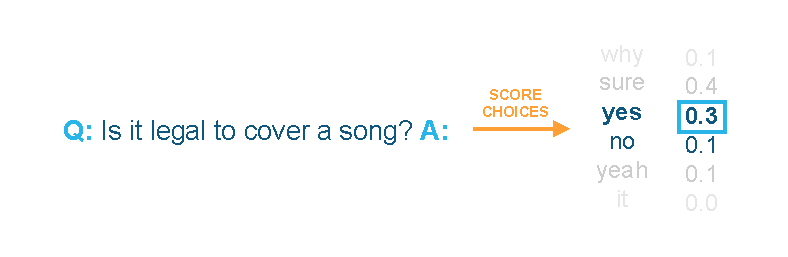
\includegraphics[width=\textwidth]{assets/pretraining_results/contamination_analysis/boolq}
    \end{subfigure}
    \begin{subfigure}[b]{0.246\textwidth}
    \includegraphics[width=\textwidth]{assets/pretraining_results/contamination_analysis/csqa}
    \end{subfigure}
    \begin{subfigure}[b]{0.246\textwidth}
    \includegraphics[width=\textwidth]{assets/pretraining_results/contamination_analysis/drop}
    \end{subfigure}
    \begin{subfigure}[b]{0.246\textwidth}
    \includegraphics[width=\textwidth]{assets/pretraining_results/contamination_analysis/gsm8k}
    \end{subfigure}
    \begin{subfigure}[b]{0.246\textwidth}
    \includegraphics[width=\textwidth]{assets/pretraining_results/contamination_analysis/hellaswag}
    \end{subfigure}
    \begin{subfigure}[b]{0.246\textwidth}
    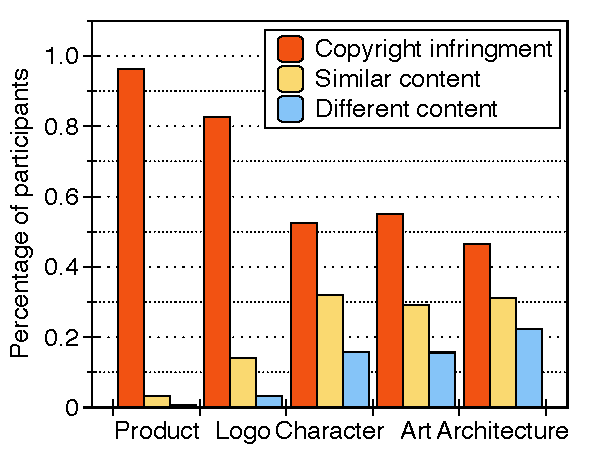
\includegraphics[width=\textwidth]{assets/pretraining_results/contamination_analysis/human_eval}
    \end{subfigure}
    \begin{subfigure}[b]{0.246\textwidth}
    \includegraphics[width=\textwidth]{assets/pretraining_results/contamination_analysis/math}
    \end{subfigure}
    \begin{subfigure}[b]{0.246\textwidth}
    \includegraphics[width=\textwidth]{assets/pretraining_results/contamination_analysis/mbpp}
    \end{subfigure}
    \begin{subfigure}[b]{0.246\textwidth}
    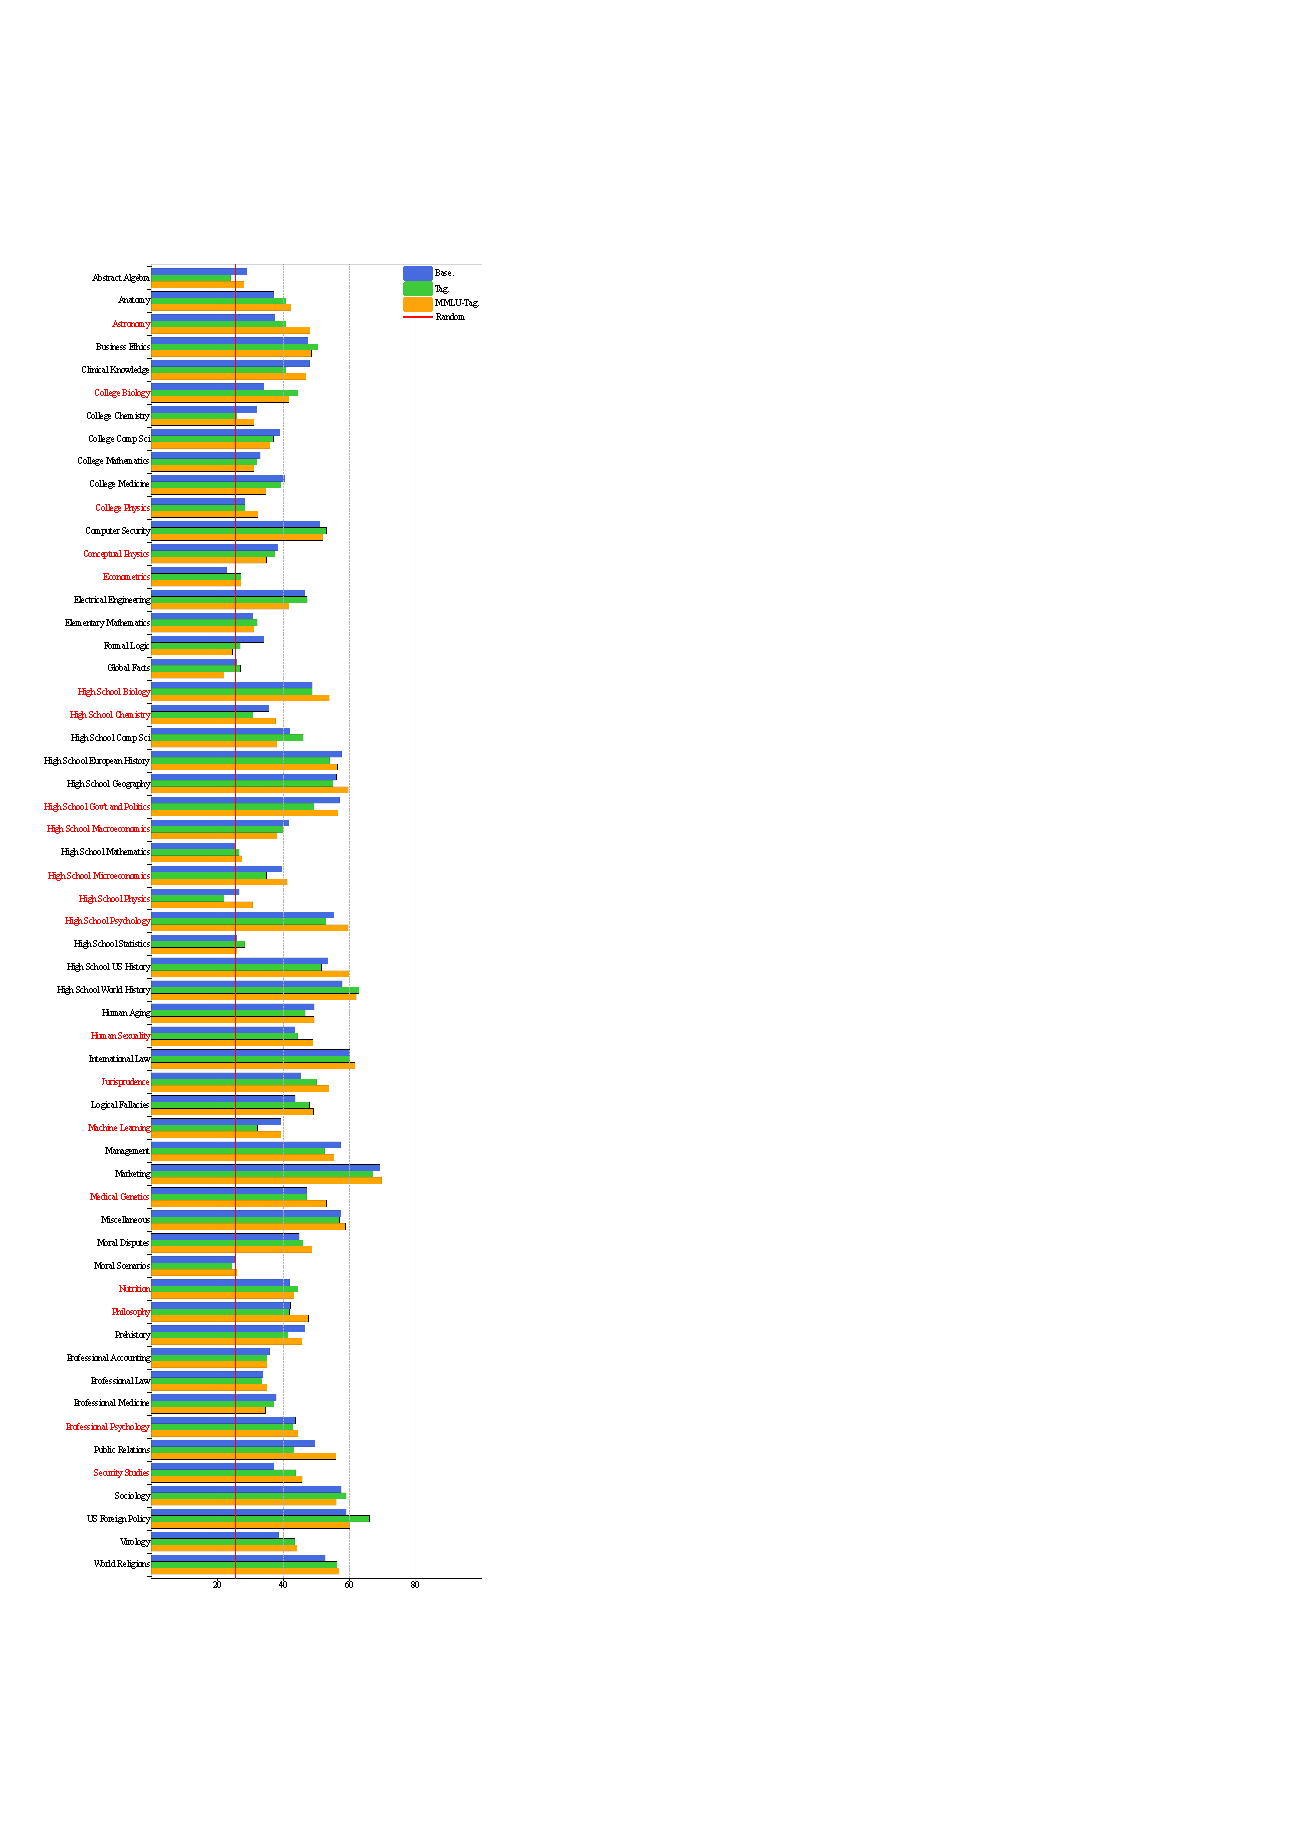
\includegraphics[width=\textwidth]{assets/pretraining_results/contamination_analysis/mmlu}
    \end{subfigure}
    \begin{subfigure}[b]{0.246\textwidth}
    \includegraphics[width=\textwidth]{assets/pretraining_results/contamination_analysis/mmlu_pro}
    \end{subfigure}
    \begin{subfigure}[b]{0.246\textwidth}
    \includegraphics[width=\textwidth]{assets/pretraining_results/contamination_analysis/nq}
    \end{subfigure}
    \begin{subfigure}[b]{0.246\textwidth}
    \includegraphics[width=\textwidth]{assets/pretraining_results/contamination_analysis/obqa}
    \end{subfigure}
    \begin{subfigure}[b]{0.246\textwidth}
    \includegraphics[width=\textwidth]{assets/pretraining_results/contamination_analysis/piqa}
    \end{subfigure}
    \begin{subfigure}[b]{0.246\textwidth}
    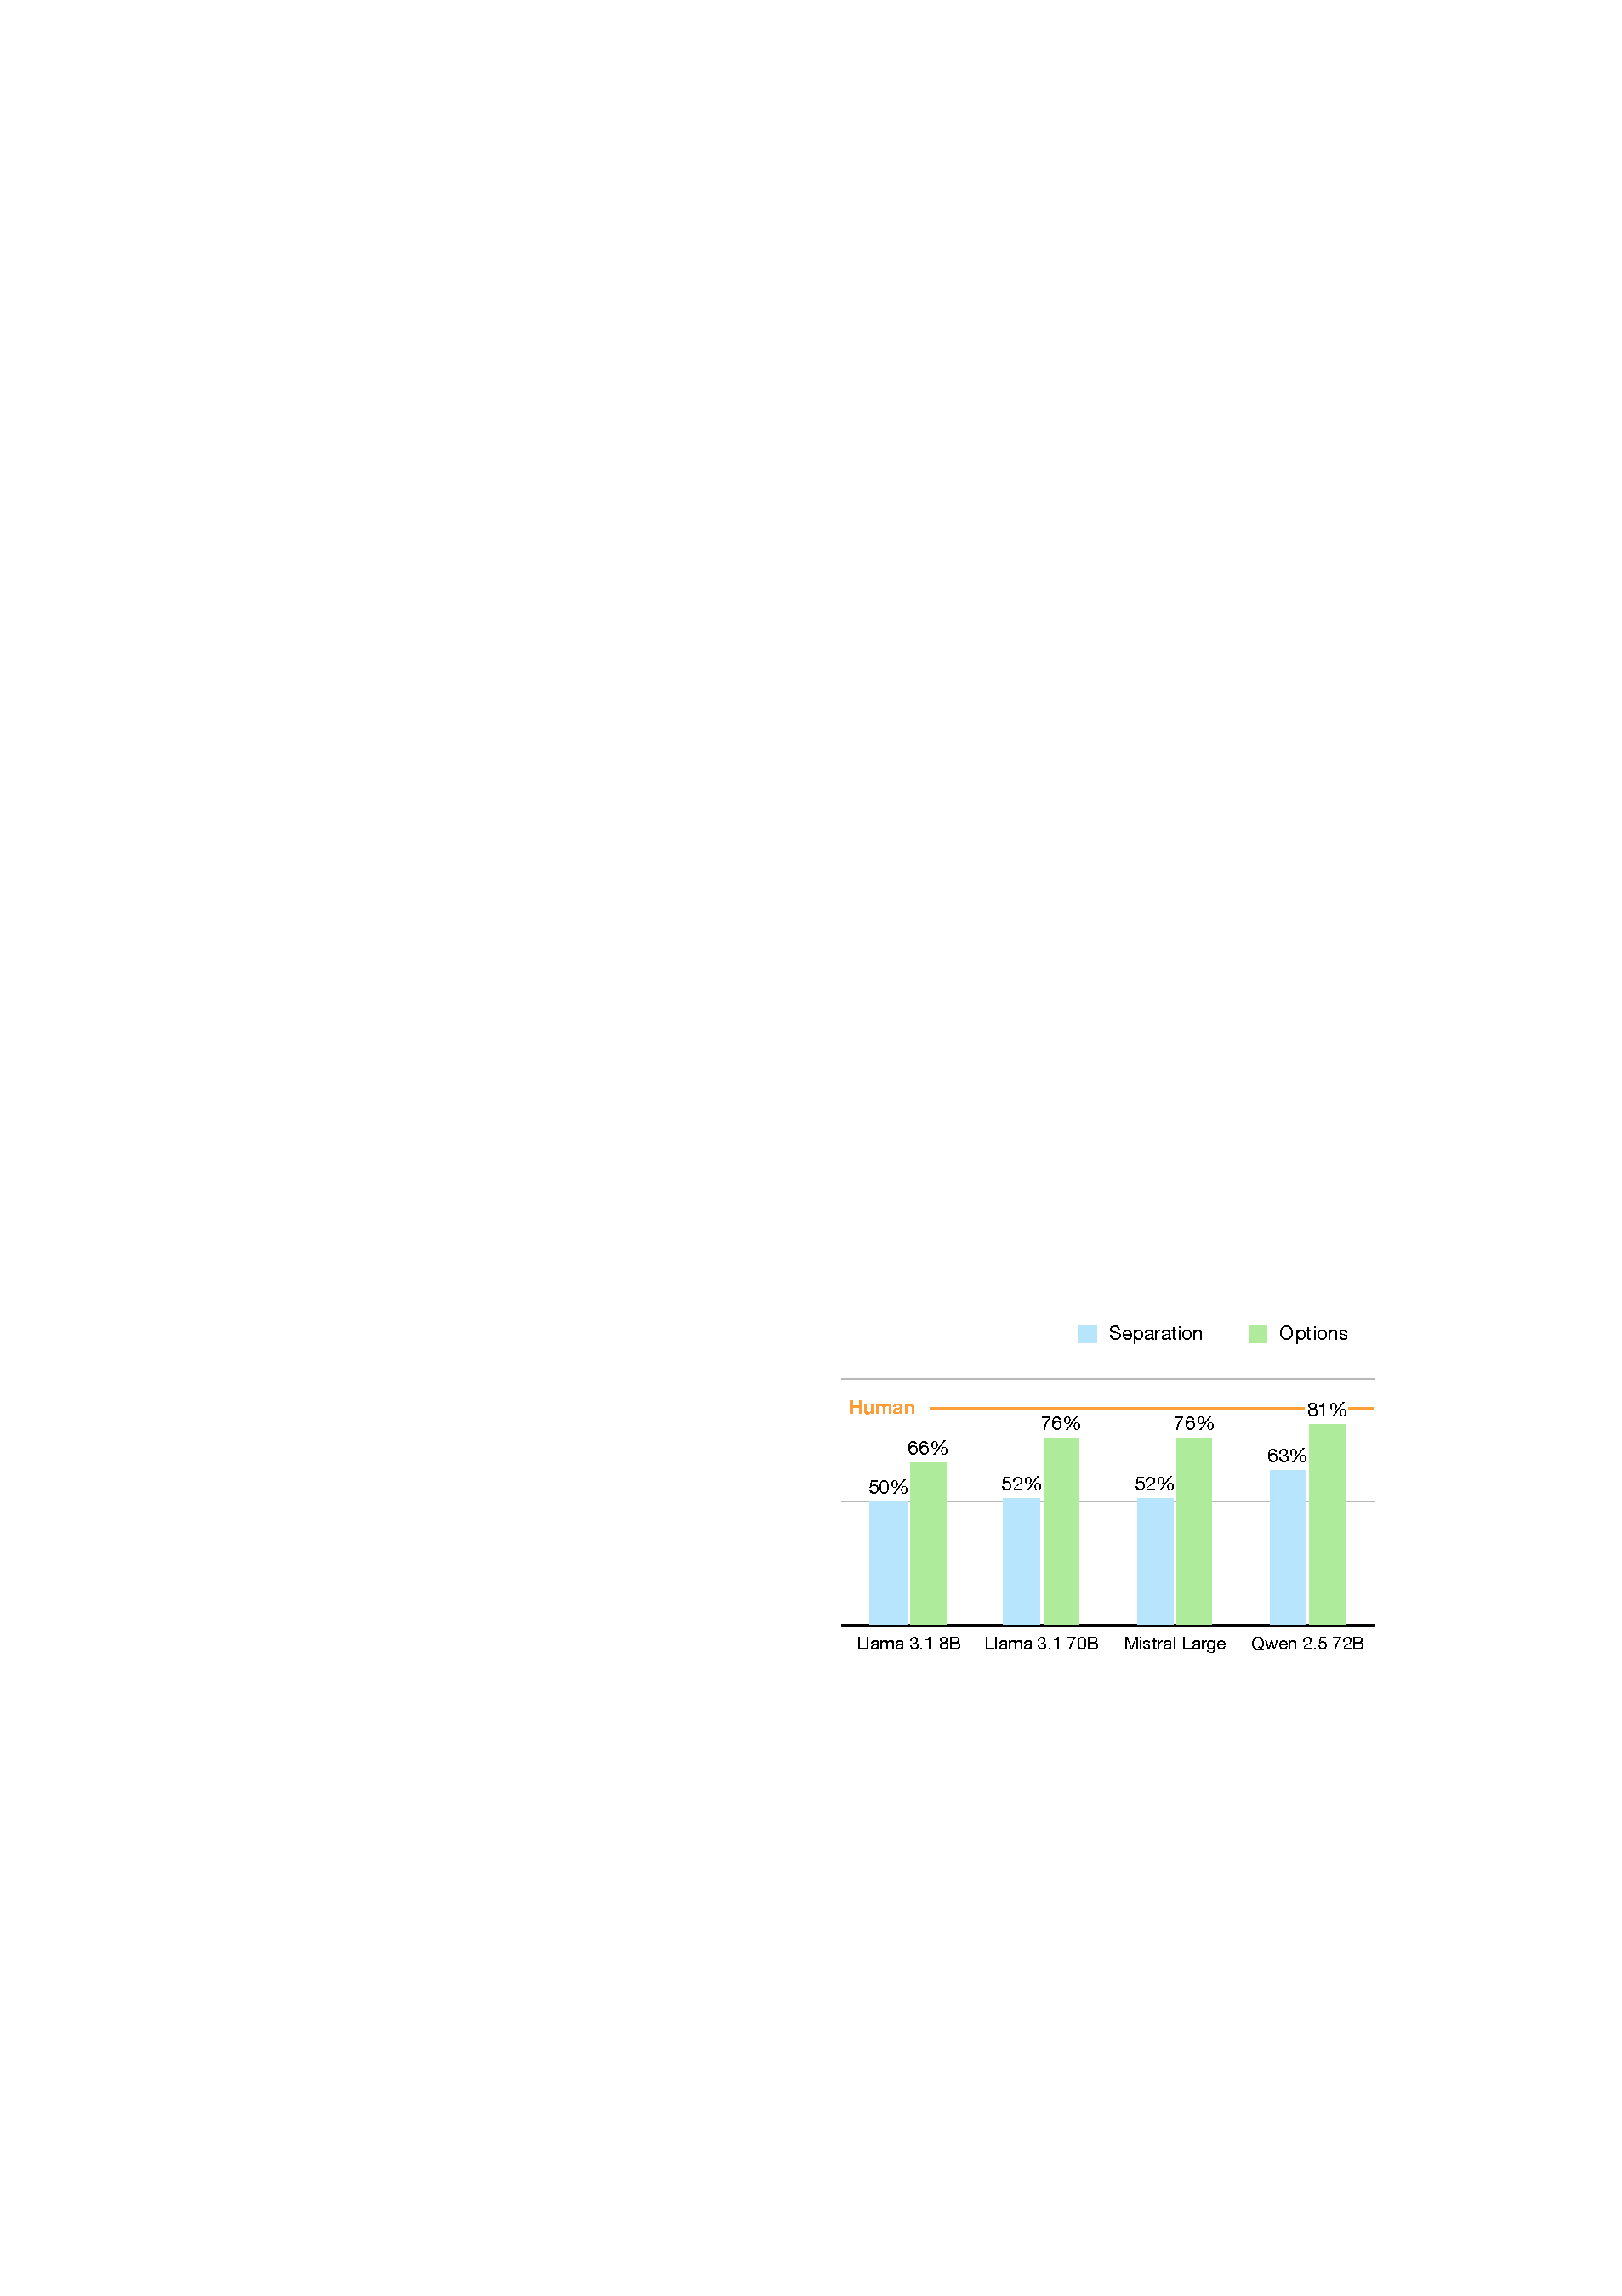
\includegraphics[width=\textwidth]{assets/pretraining_results/contamination_analysis/siqa}
    \end{subfigure}
    \begin{subfigure}[b]{0.246\textwidth}
    \includegraphics[width=\textwidth]{assets/pretraining_results/contamination_analysis/squad}
    \end{subfigure}
    \begin{subfigure}[b]{0.246\textwidth}
    \includegraphics[width=\textwidth]{assets/pretraining_results/contamination_analysis/winogrande}
    \end{subfigure}
    \begin{subfigure}[b]{0.246\textwidth}
    \includegraphics[width=\textwidth]{assets/pretraining_results/contamination_analysis/worldsense}
    \end{subfigure}
    \caption{Estimation of performance gain and estimated contamination per threshold.}\label{figure:contamination_analysis}
\end{figure}
